
%(BEGIN_QUESTION)
% Copyright 2013, Tony R. Kuphaldt, released under the Creative Commons Attribution License (v 1.0)
% This means you may do almost anything with this work of mine, so long as you give me proper credit

Suppose you are asked to configure the instruments in this pressure control loop to sense and display process pressure over a range of 0 to 150 kPa, with the loop controller actuating two split-ranged control valves in a progressive sequence:

$$\includegraphics[width=15.5cm]{i02081x01.eps}$$

Write the proper range values inside the boxes near each instrument, showing the proper configuration for each instrument needed to achieve the desired result.

\vskip 20pt \vbox{\hrule \hbox{\strut \vrule{} {\bf Suggestions for Socratic discussion} \vrule} \hrule}

\begin{itemize}
\item{} Suppose the controller displayed a pressure of 80 kPa when the actual process pressure was 87 kPa PSIG.  First, identify {\it two} possible locations in this loop for a calibration error that would account for this discrepancy.  Then, assuming only one fault, explain how you could positively determine the location of this calibration error with a single diagnostic test.
\item{} Suppose valve PV-A was 100\% open and PV-B was 60\% open when the controller output displayed 75\%.  First, identify {\it three} possible locations in this loop for a calibration error that would account for this discrepancy.  Then, assuming only one fault, explain how you could positively determine the location of this calibration error with no more than two diagnostic tests.
\end{itemize}

\underbar{file i02081}
%(END_QUESTION)





%(BEGIN_ANSWER)

This ranges shown here for split-ranging the two control valves do not constitute the only possible range values that will work!

$$\includegraphics[width=15.5cm]{i02081x02.eps}$$

Try to identify what {\it other} I/P and control valve positioner range values will also yield the desired split-range sequencing.

%(END_ANSWER)





%(BEGIN_NOTES)

A PV measurement error could lie within the transmitter, or within the controller's analog input.  A single current measurement of the transmitter's signal will tell you where the calibration error resides.

\vskip 10pt

A valve positioning error affecting PV-B (PV-A could also be affected, but we do not know because it's supposed to be saturated at 100\% at this controller output value) could lie within PV-B's positioner or the PY-B I/P transducer.  A pressure measurement at the PY-B I/P output will tell you if a calibration error resides in the valve positioner.  Comparing this pressure measurement against a measurement of controller output current will tell you if a calibration error resides in that I/P.

%INDEX% Basics, transmitter: input and output ranges
%INDEX% Final Control Elements, valve: split ranging

%(END_NOTES)

